\documentclass[../TDON2_inter.tex]{subfiles}%

\begin{document}
\section[s]"2"{Mesure de l'épaisseur d'une lame de verre}

\enonce{%
	On considère un dispositif de trous d'\textsc{Young} composé de deux trous $T_1$
	et $T_2$ séparés d'une distance $a = \SI{100}{\micro m}$. Ce dispositif est
	éclairé par une source ponctuelle S monochromatique de longueur d'onde dans
	l'air $\lambda = \SI{532}{nm}$ située sur l'axe optique. La figure
	d'interférences est observée sur un écran situé à une distance $D =
		\SI{1.00}{m}$ du plan des trous. Une lame de verre à faces parallèles
	d'épaisseur $e$ inconnue et d'indice $n_v = \num{1.57}$ est positionnée en
	sortie du trou $T_1$. L'indice optique de l'air est supposé égal à 1.

	\begin{center}
		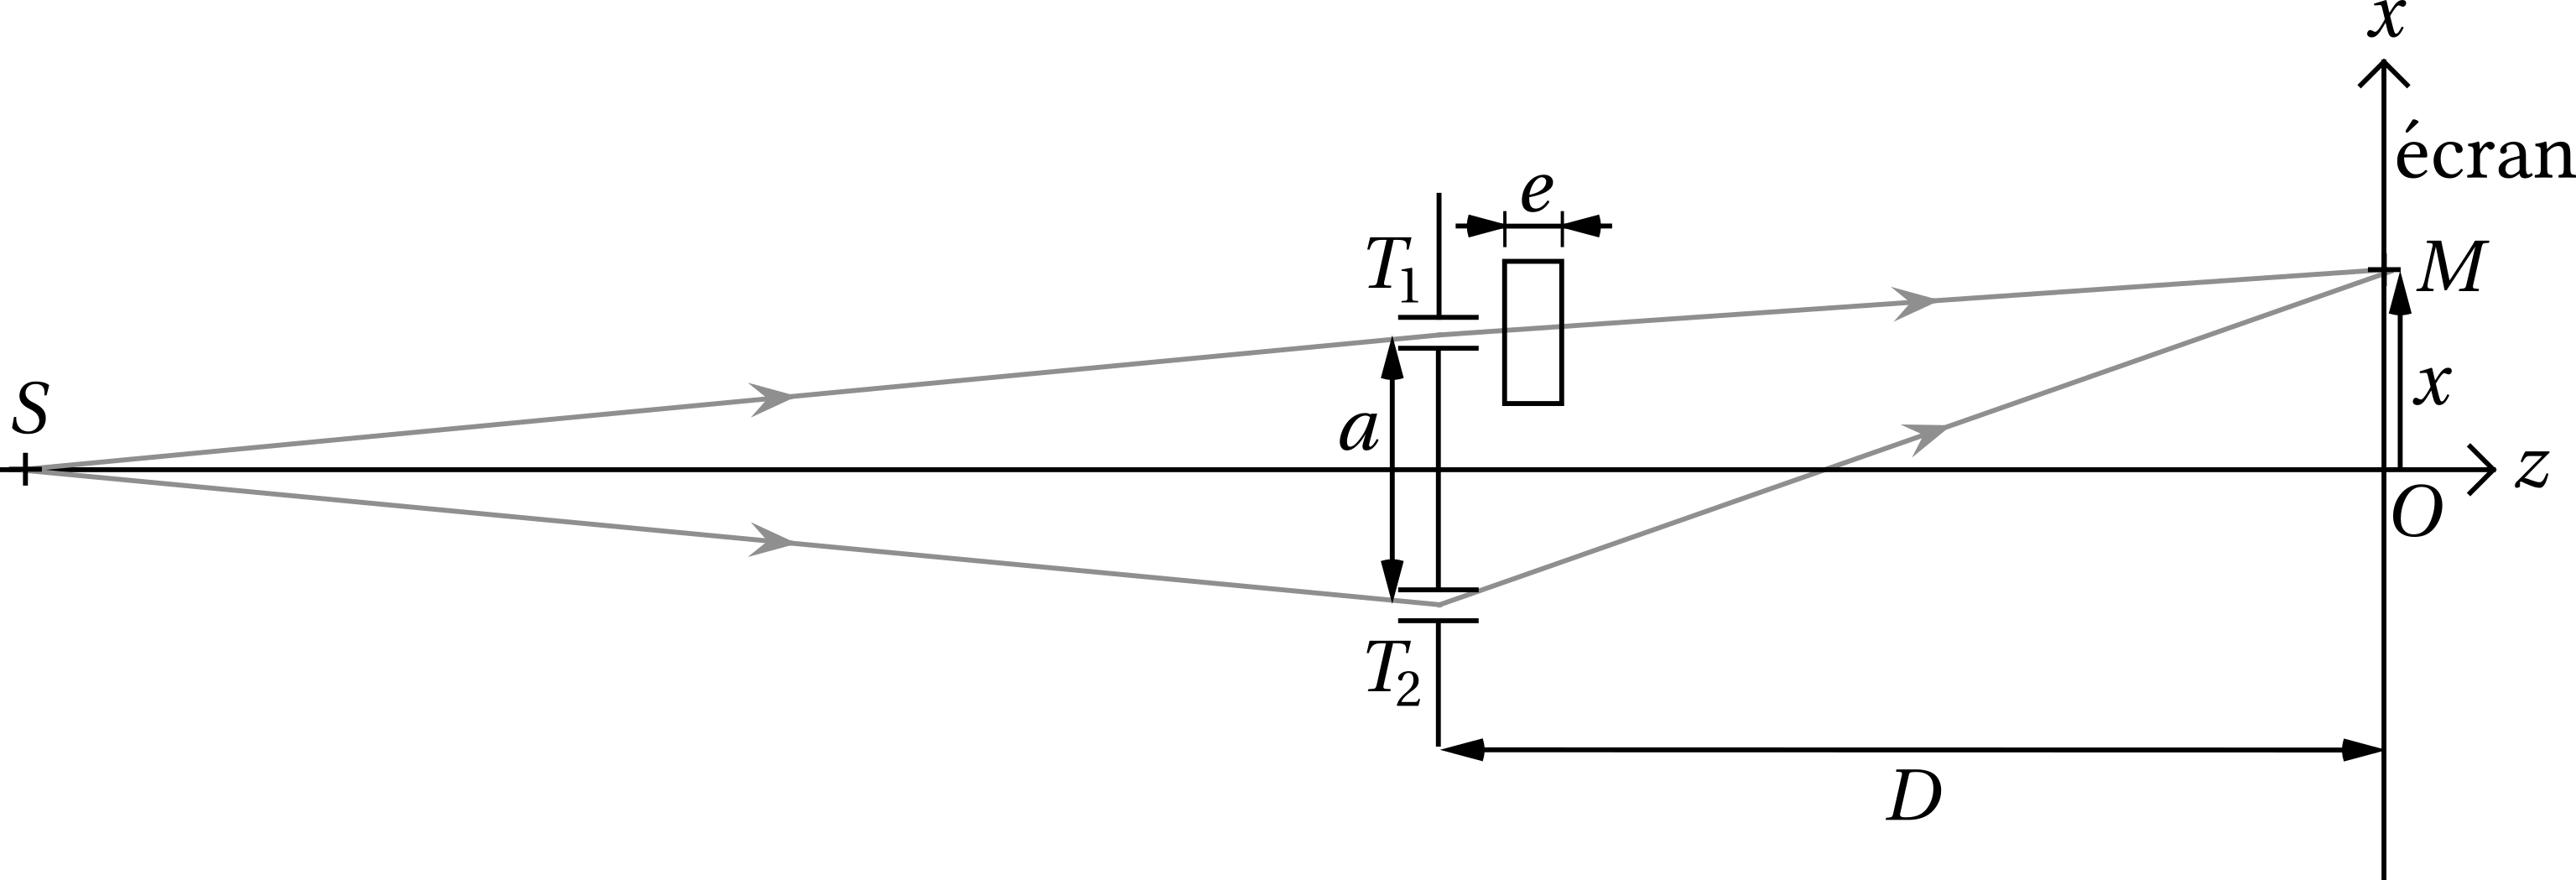
\includegraphics[width=0.8\linewidth]{lame_verre-plain}
	\end{center}
}

\QR{%
	Montrer que la différence de chemin optique $\delta(\Mr)$ en un point M de
	l'écran s'écrit
	\[\delta(\Mr) = \frac{ax}{D} - (n_v - 1)e\]
}{%
	En notant $({\rm SM})$ le chemin optique de S à M, la différence de
	chemin optique en M est donnée par
	\begin{gather*}
		\de_{2/1}(\Mr)
		= \rm (ST_2M) - (ST_1M)
		= \rm \cancel{\rm (ST_2)} + (T_2M) - \cancel{\rm (ST_1)} - (T_1M)
	\end{gather*}
	La source étant sur l'axe optique et l'indice étant le même sur cette
	portion, on a \fbox{$\rm (ST_1) = (ST_2)$}. On se retrouve donc à calculer le
	chemin optique à partir des trous. Or, le chemin de T$_2$ à $M$ se fait
	dans l'air, donc \fbox{(T$_2$M) = T$_2$M}. En notant F$_1$ et F$_2$ les
	points d'entrée et de sortie du rayon lumineux dans la lame de verre
	tels que ${\rm F_1F_2}=e$, on a
	\begin{align*}
		({\rm T_1M})
		 & = \rm (T_1F_1) + (F_1F_2) + \rm (F_2M)                 \\
		 & = {\rm T_1F_1} + n_ve + {F_2M}                         \\
		 & = {\rm T_1F_1} + n_ve + {\rm F_1F_2-F_1F_2} + \rm F_2M \\
		 & = {\rm T_1F_1 + F_1F_2 + F_2M} + (n_v-1)e              \\
		 & = {\rm T_1M} + (n_v-1)e
	\end{align*}
	Avec $\rm T_1M = T_1F_1+F_1F_2+F_2M$. Autrement dit,
	\begin{gather*}
		\de_{2/1}(\Mr) = {\rm T_2M - T_1M} - (n_v-1)e
	\end{gather*}
	et avec le résultat usuel de différence de marche des trous
	d'\textsc{Young}, c'est-à-dire $\D L_{2/1}(\Mr) = ax/D$ (attention à la
	notation de la distance entre les fentes~!), on trouve bien
	\[\boxed{\de_{2/1}(\Mr) = \frac{ax}{D} - (n_v-1)e}\]
	Autrement dit, la différence de chemin optique est celle sans la lame à
	laquelle s'ajoute le retard pris par l'onde issue de T$_1$ qui va moins
	vite/parcourt une plus grande distance (à la célérité $c$) à cause du verre.
	On retrouve bien que si $n_v = 1$, la différence de chemin optique est celle
	attendue sans lame de verre.
}

\QR{%
	Déterminer la position $x_c$ sur l'écran de la frange centrale
	correspondant à $\delta(\Mr) = 0$. De quelle distance s'est déplacée
	cette frange par rapport au cas où la lame est absente~?
}{%
	\leavevmode\vspace*{-25pt}\relax
	\begin{gather*}
		\de_{1/2}(\Mr) = 0
		\Lra
		\frac{ax_c}{D} - (n_v-1)e = 0
		\Lra
		\boxed{x_c = \frac{(n_v-1)eD}{a}}
	\end{gather*}
	En l'absence de la lame de verre, la frange centrale serait sur l'axe
	optique, en $x = 0$~: dans cette situation, elle s'est donc décalée de
	$x_c$.
}

\QR{%
	Exprimer l'épaisseur $e$ de la lame en fonction de $x_c$ , $a$, $n_v$
	et $D$, puis calculer $e$ pour $x_c = \SI{28.5}{cm}$.
}{%
	\leavevmode\vspace*{-25pt}\relax
	\begin{gather*}
		\beforetext{On isole~:}
		\boxed{e = \frac{ax_c}{D(n_v-1)}}
		\qavec
		\left\{
		\begin{array}{rcl}
			a   & = & \SI{100}{\micro m}    \\
			D   & = & \SI{1.00e9}{\micro m} \\
			n_v & = & \num{1.57}            \\
			x_c & = & \SI{28.5e7}{\micro m}
		\end{array}
		\right.\\
		\AN
		\xul{%
			e = \SI{50.0}{\micro m}
		}%
	\end{gather*}
}

\QR{%
	Expliquer pourquoi en réalité la position de la frange centrale ne
	peut être connue que modulo l'interfrange $i$. Qu'est-ce que cela
	implique sur $e$~? L'expérience vous paraît-elle réalisable~?
}{%
	La frange centrale, en première approximation, n'est pas distinguable
	des autres franges brillantes correspondant également à des
	interférences constructives~: on a donc sa position modulo
	l'interfrange, soit
	\[x_c \equiv x_c \quad \left[ \frac{\lambda D}{a} \right]\]
	et ainsi
	\[e \equiv e \quad \left[ \frac{\lambda}{n_v-1} \right]\]
	Autrement dit, la mesure de $e$ n'est possible que modulo
	$\lambda/(n_v-1) = \SI{0.9}{\micro m}$~: la mesure de la lame de verre
	ne serait donc pas réalisable avec cette expérience, puisqu'elle est
	plus grande que \SI{0.9}{\micro m}.
	\smallbreak
	Dans la pratique, la frange brillante principale est distinguable des autres
	par atténuation de la luminosité sur les bords, donc l'expérience fonctionne.
}
\end{document}
